\section{Results}
\label{sec:4.2_results}

% 4.2.1
% -----
\subsection{Network overview}
\label{sec:4results_overview}

To train a CNN to predict the fluorescence signal from EM images, we create training datasets comprised of high-magnification EM and FM image pairs. The FM images are acquired by a fluorescence microscope integrated into the chamber of a scanning electron microscope (SEM) \cite{liv2013simultaneous, zonnevylle2013integration}. This experimental setup allows for high accuracy overlay precision without a reliance on fiducial markers or manual input \cite{haring2017automated}. This is advantageous as it prevents the network from learning on extrinsic markers or bias in the image registration. It further allows for the semi-automated accumulation of correlative datasets, scalable to several GBs \cite{lane2021optimization}.

To optimize performance for GPU clusters, the large-scale correlated datasets are divided into small tiles which serve as input for the model (Figure \ref{fig:4.1_overview}A). Image tiles are shuffled to diversify the training area, reducing the likelihood of overfitting to a particular region of the specimen. A deep CNN was chosen for the model architecture for its strength in recognizing structural detail in EM images as well as for its superhuman pattern recognition capabilities \cite{cciccek20163d}. To address the resolution mismatch between EM-FM image pairs, the model is designed with more contraction than expansion paths, which results in an elongated, backwards ``J"-shape as opposed to the more typical ``U" (Figure \ref{fig:4.1_overview}B). Once trained, the model is able to generate predictions of the fluorescence intensity on individual EM image tiles. Separate correlative EM-FM datasets are set aside for validating and testing the model. By stitching together the model's output it is possible to render large-scale predictions of the fluorescence intensity, which can then be overlaid onto the EM test dataset (Figure \ref{fig:4.1_overview}C).

% Figure 4.1 (overview)
% ---------------------
\begin{figure}[!tb]
    \centering
    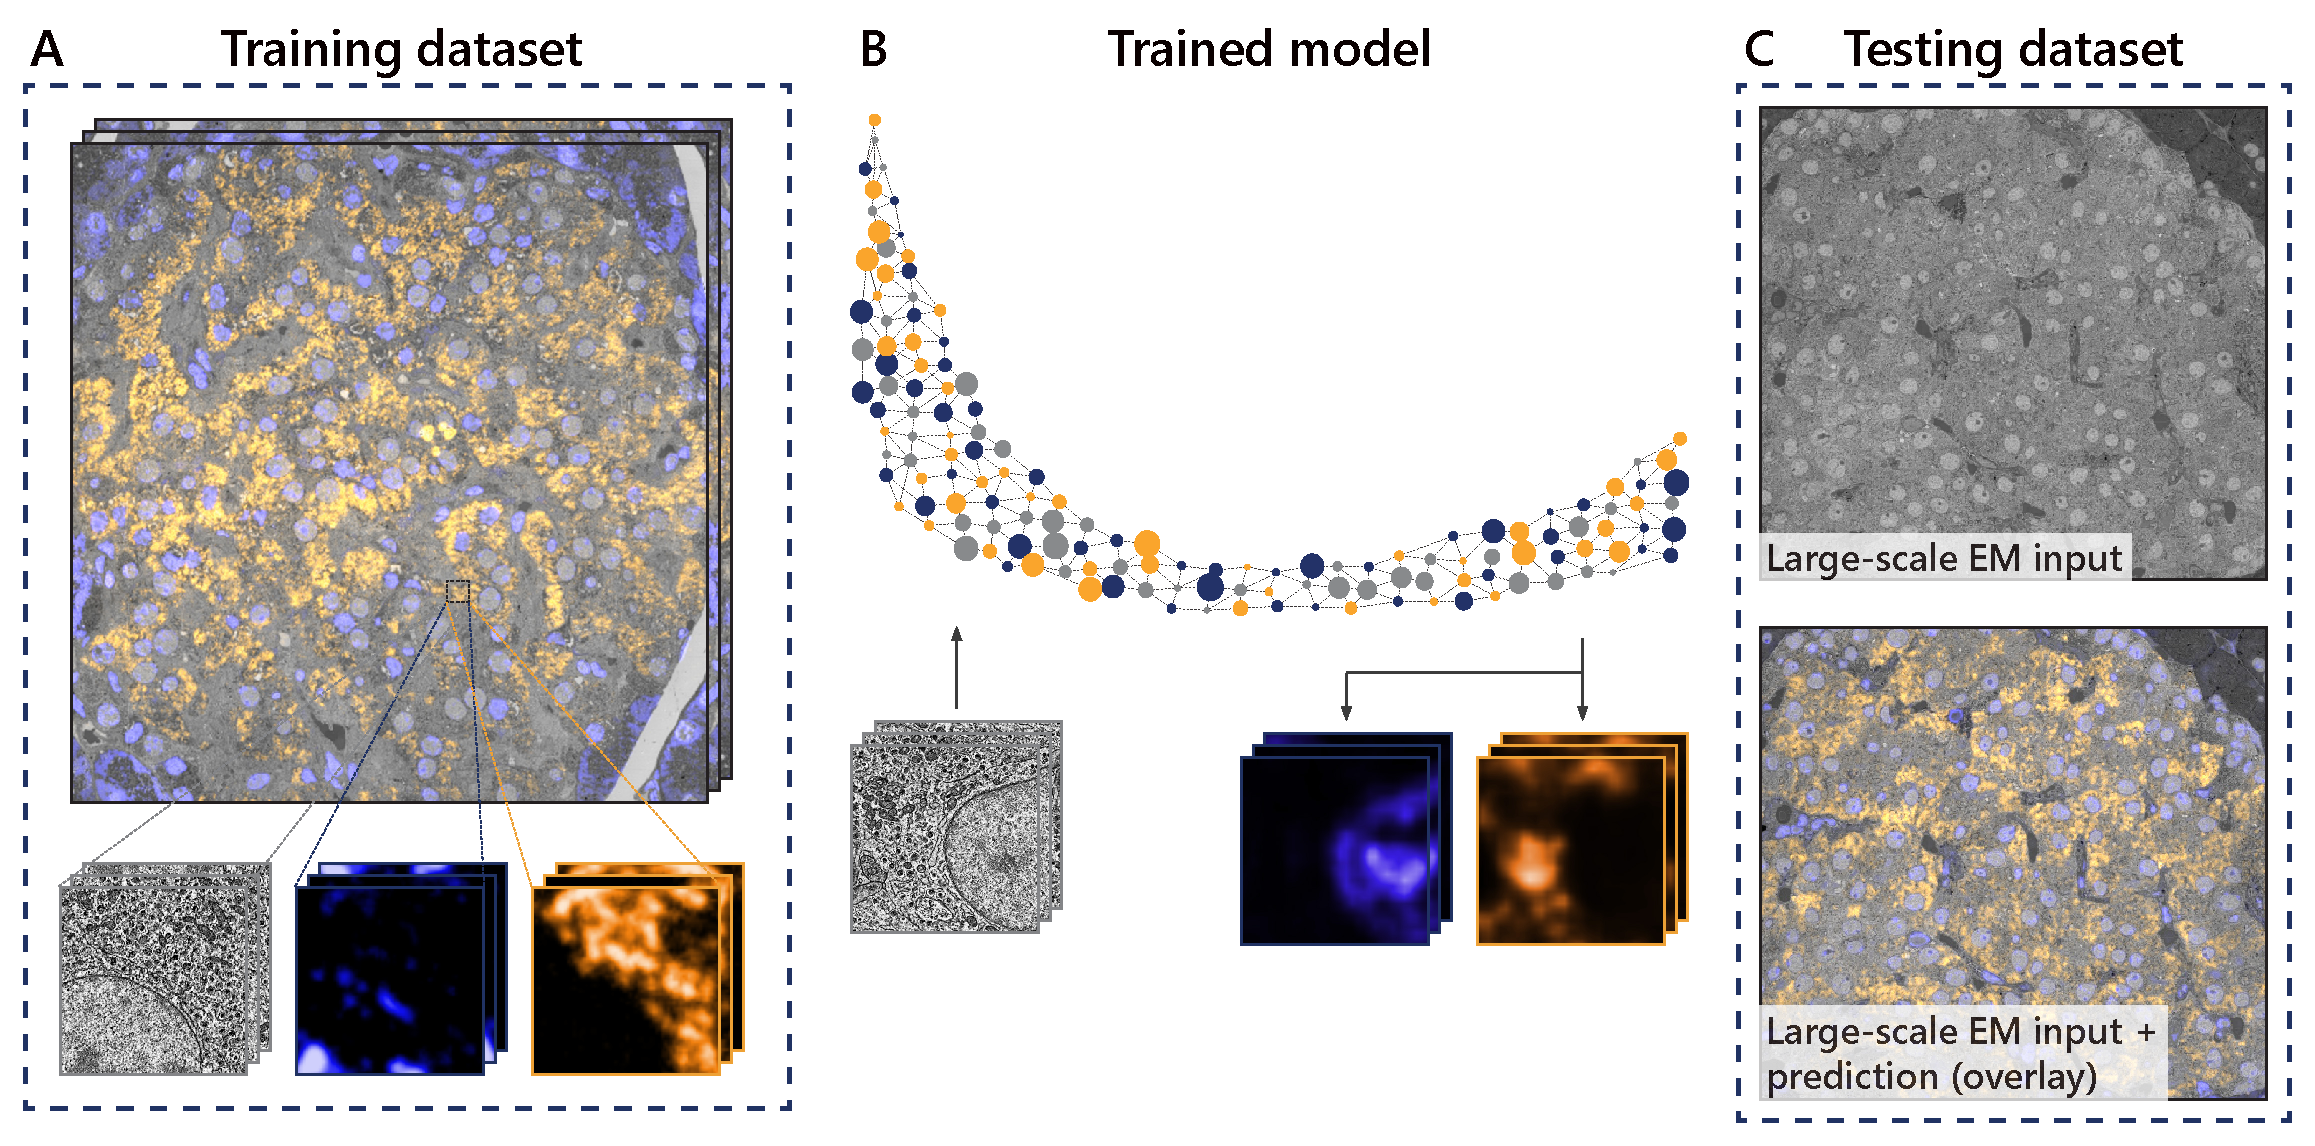
\includegraphics[width=\linewidth]{chapter-4/figures_PDF/fig4-1_overview.pdf}
    \caption{Procedure for fluorescence intensity predictions.
    (A) Training data for the model consists of registered, large-scale CLEM datasets. For the rat pancreas tissue shown here, the fluorescent channels consist of a Hoechst stain (blue), targeting cell nuclei, and AF594 (orange), immuno-targeted to insulin granules.
    (B) The correlative image data is input to an asymmetric convolutional neural network which maps EM to FM. The model is illustrated as a backwards ``J" due to the resolution mismatch between EM and FM.
    (C) Once trained, the network generates predictions on EM test data such that the predictions can be overlaid to amass large-scale, artificial CLEM datasets.}
    \label{fig:4.1_overview}
\end{figure}


% 4.2.2
% -----
\subsection{Network predictions on thin tissue sections}
\label{sec:4results_pancreas}

To characterize the performance of our network, we first apply it to routinely prepared ultrathin sections of rat pancreas tissue \cite{ravelli2013destruction}. The sections are stained with Hoechst, targeting cell nuclei, and immunolabelled with AF594, targeting insulin granules. The prediction (green) is found to correlate well with the measured fluorescence (red); PCCs of 0.67 for Hoechst (Figure \ref{fig:4.2_pancreas}A) and 0.76 for AF594 (Figure \ref{fig:4.2_pancreas}F) are computed when averaged across an entire islet of Langerhans. At high magnification, the measured and predicted intensities for Hoechst are found to exhibit a close qualitative resemblance ($\rho\!=\!\text{0.73}$; Figure \ref{fig:4.2_pancreas}B--E). Notably, both signals are more heavily concentrated along the nuclear envelope and areas of denser chromatin within the nucleus. The predicted AF594 signal matches well with that of the measured fluorescence ($\rho\!=\!\text{0.73}$; Figure \ref{fig:4.2_pancreas}H--J) with the caveat that the predicted intensity appears to spread out more uniformly over adjacent insulin granules---possibly due to the granules being diffraction-limited.

% Figure 4.2 (pancreas)
% ---------------------
\begin{figure}[!tb]
    \centering
    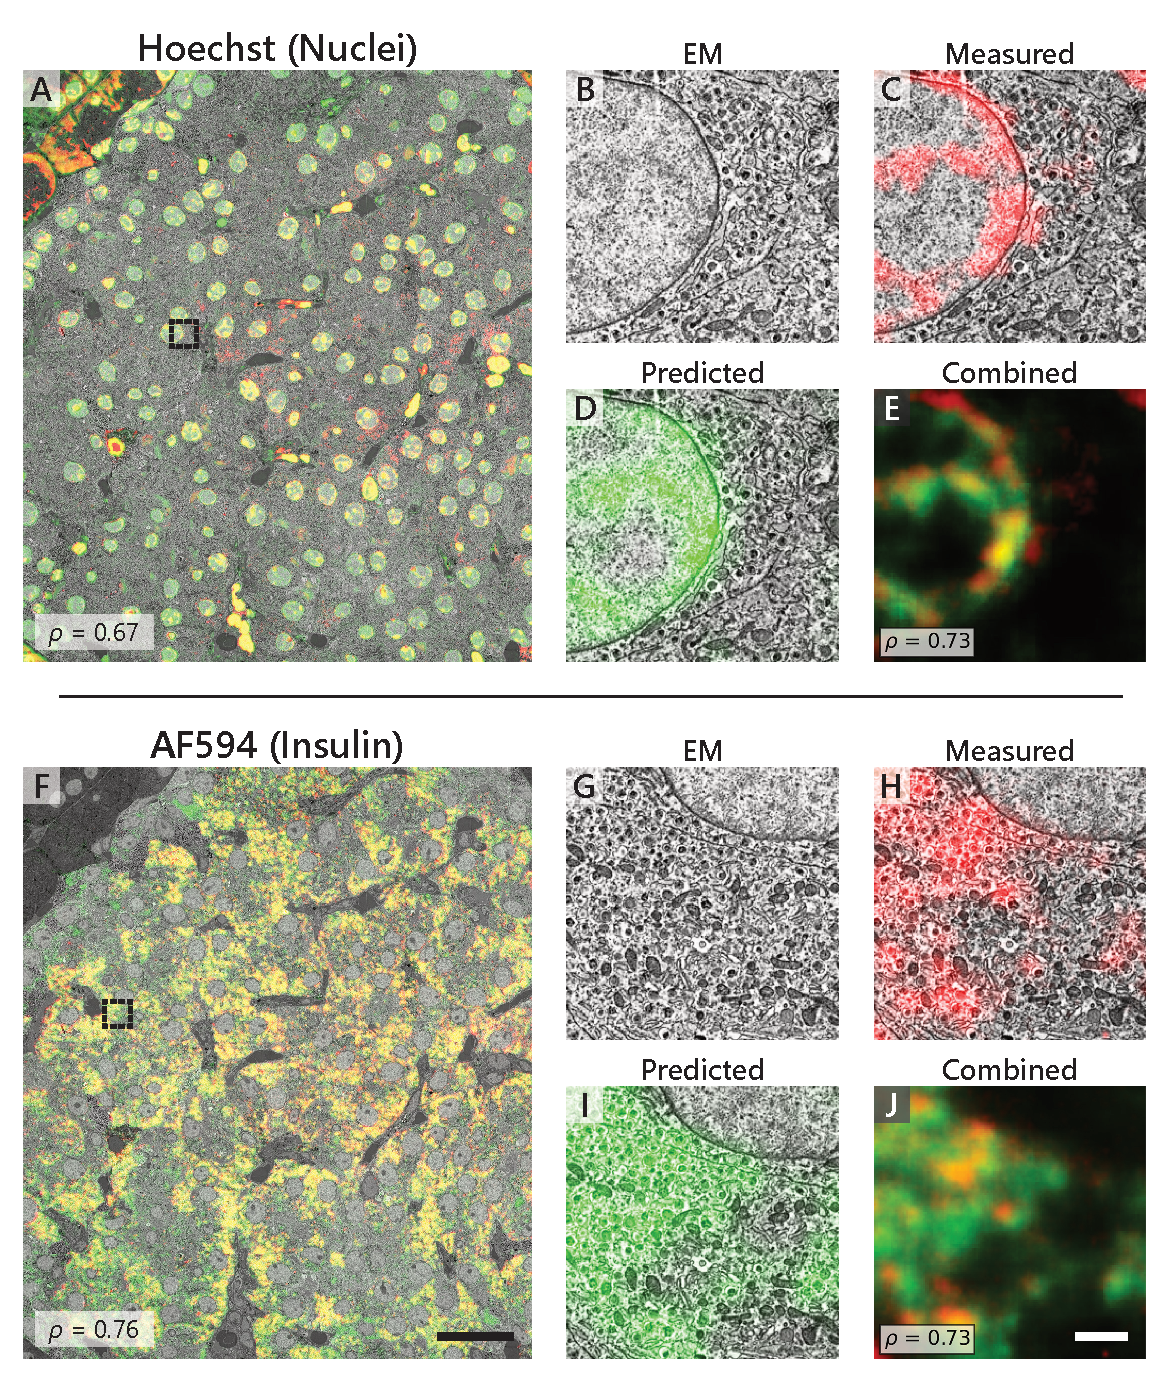
\includegraphics[width=\linewidth]{chapter-4/figures_PDF/fig4-2_pancreas.pdf}
    \caption{Network predictions of the fluorescence intensity correlate well with the measured fluorescence signal.
    (A) The measured (red) and predicted (green) fluorescence for a nucleus marker overlaid onto a large-scale EM dataset of an islet of Langerhans. Regions of high correlation appear as yellow. 
    Zoomed insets show the EM (B); measured (C), predicted (D), and combined (E) fluorescence for an individual cell nucleus.
    (F) Same as in (A) but for AF594 targeting insulin granules.
    (G\,--\,J) Same as in (B\,--\,E) but for a cluster of insulin granules.
    Scale bars: (A, F) \SI{20}{\micro\meter}; (B\,--\,E, G\,--\,J) \SI{1}{\micro\meter}.}
    \label{fig:4.2_pancreas}
\end{figure}

There are other factors that may contribute to a diminished PCC that are extraneous to the network. These include bleedthrough of one fluorescence channel into another (Figure \ref{fig:4.S1_rois}B), errors in the EM-FM registration (Figure \ref{fig:4.S1_rois}C), and aberrations in the fluorescence microscope (Figure \ref{fig:4.S1_rois}D). Not only do these cases warrant a reduced correlation coefficient, but they demonstrate the network's ability to effectively correct for imperfections in the measured fluorescence.


% 4.2.3
% -----
\subsection{Human evaluation of fluorescence vs label-free prediction}
\label{sec:4results_evaluation}

To further characterize the performance of the model, we assess human recognition of cell nuclei in the network-generated predictions versus the measured fluorescence (Figure \ref{fig:4.3_counting}). In order to quantify recognition proficiency, we establish a ground truth (GT) set of cell nuclei based on EM (Figure \ref{fig:4.3_counting}A). Approximately 200 cell nuclei were manually annotated by a combination of experts and trained volunteers. Spurious annotations were filtered out using unsupervised, brute-force nearest neighbors. $k$-means clustering was then used to partition the remaining annotations into point clouds from which the centroids were computed and added to the GT.

The experts and trained volunteers were then asked to recognize cell nuclei in the measured and predicted fluorescence datasets (Figure \ref{fig:4.3_counting}B--C). Nuclei are considered to be correctly identified (true positive, TP) when they are detected within a certain threshold distance---approximately the average radius of a nucleus---from a nucleus in the GT. Incorrectly identified nuclei (points for which there is no nearby nucleus) are considered to be false positives (FP), while those that are missed entirely are considered to be false negatives (FN).

The precision, recall, and Sørensen–Dice index (F1 score) are calculated for each of the expert and trained volunteer annotation sets (Figure \ref{fig:4.3_counting}C). Similar average precision scores for the measured and predicted fluorescence (72\% vs 74\%) suggest that a comparable number of false positives were identified in both, while the notably higher recall for the predicted dataset (80\% vs 58\%) indicates that a substantially higher number of cell nuclei become recognizable from the predicted signal. This is visibly apparent throughout the dataset (Figure \ref{fig:4.3_counting}B--C insets), but is particularly noticeable in the periphery where the fluorescence is marginally weaker due to non-uniform illumination and nuclei become obscured due to Hoechst expression from RNA in the endoplasmic reticulum. The F1 scores (76\% predicted vs 64\% measured) reveal the improved recognition ability afforded by the network-generated predictions. The same assessment cannot be done for insulin granules as the typical size is {$\sim$}\SI{100}{\nano\meter}---well below the diffraction limit.

% Figure 4.3 (counting)
% ---------------------
\begin{figure}[!tb]
    \centering
    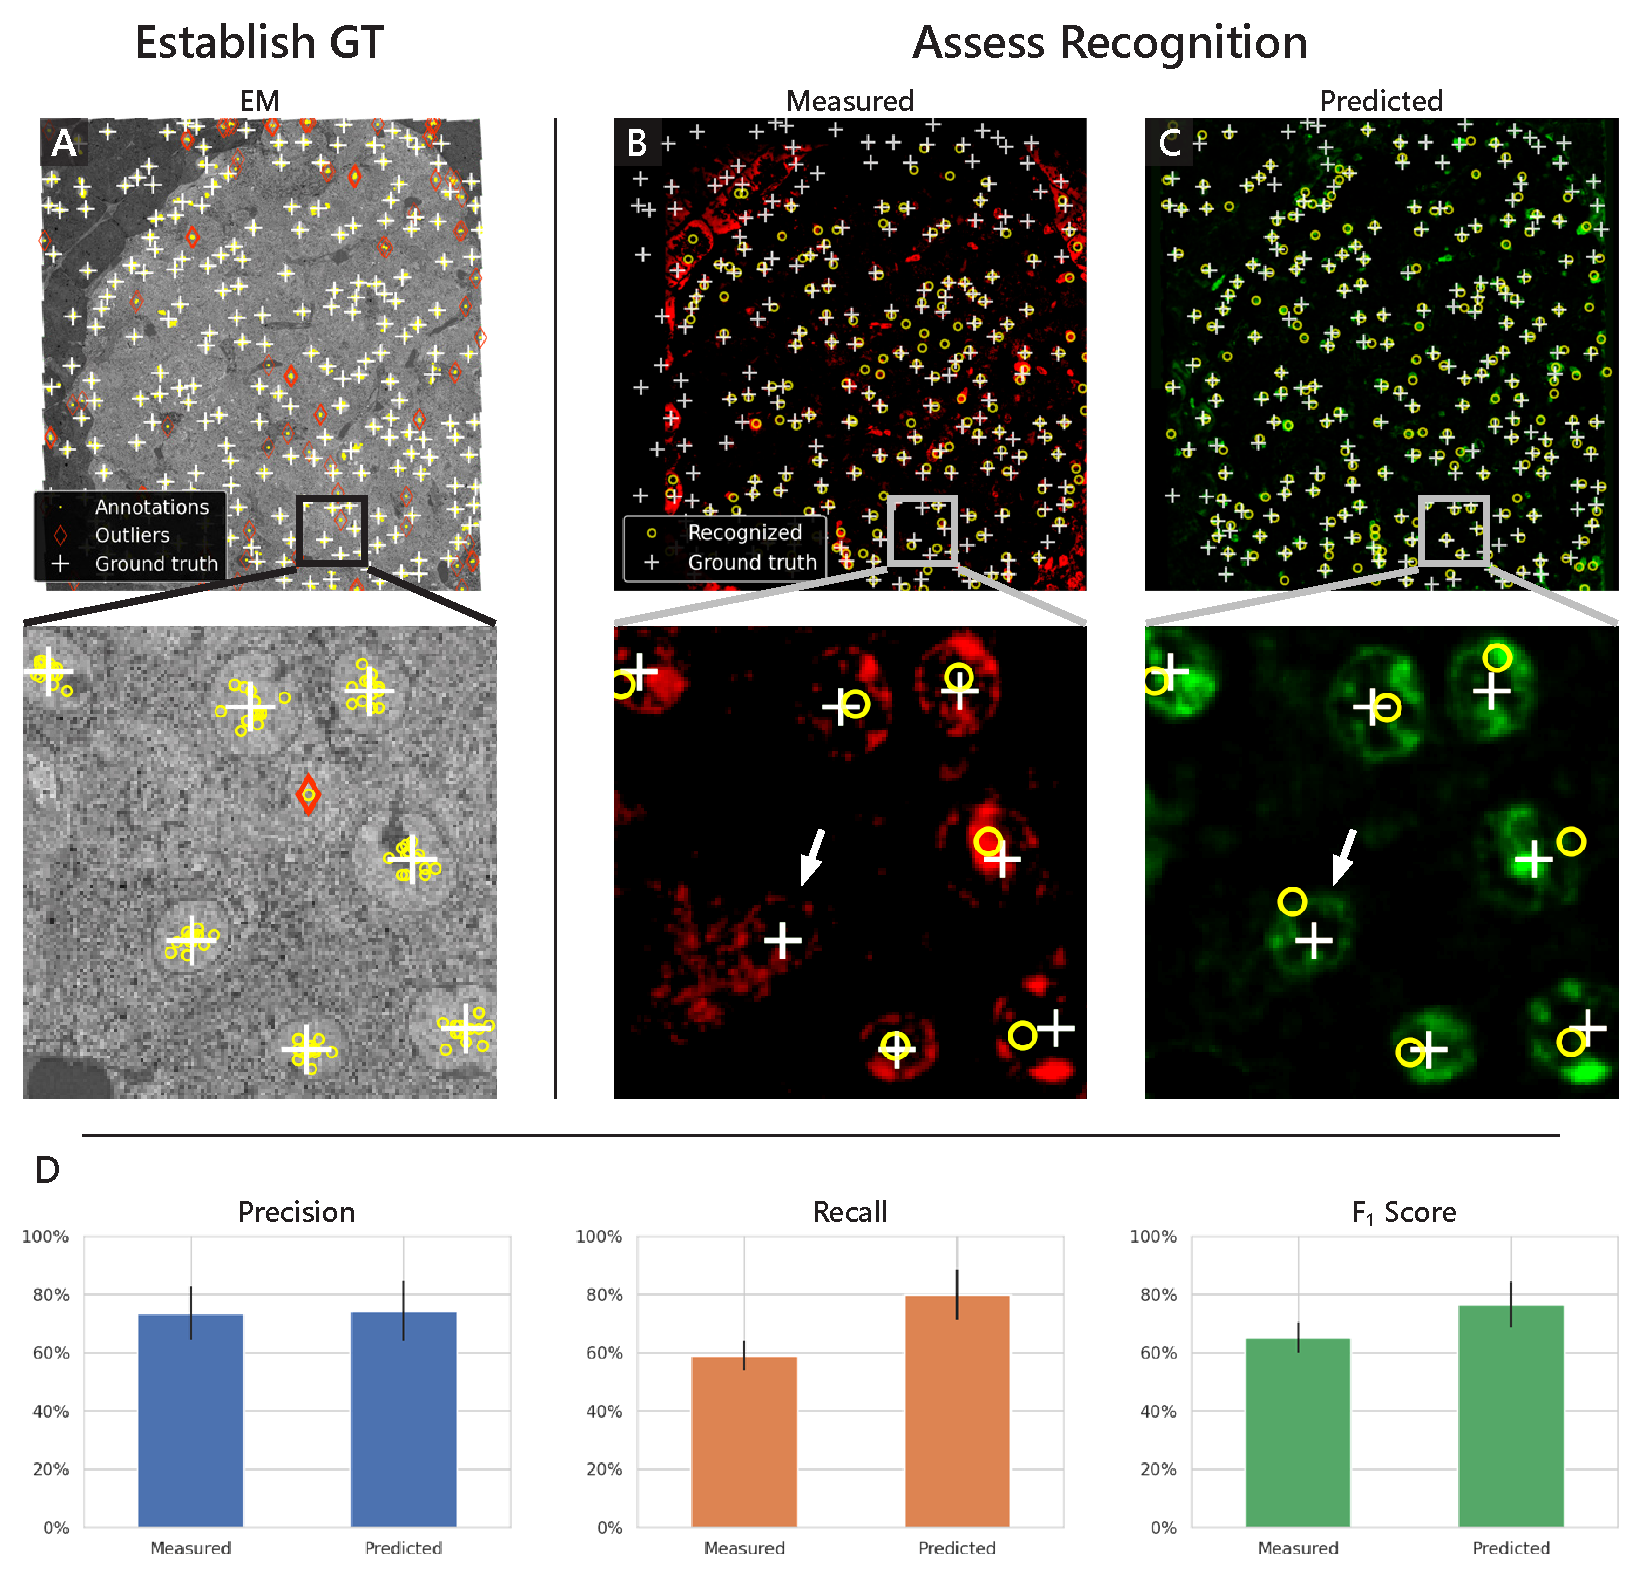
\includegraphics[width=\linewidth]{chapter-4/figures_PDF/fig4-3_counting.pdf}
    \caption{Network-generated predictions facilitate human recognition of cell nuclei.
    (A) Annotations (yellow circles) of EM data are aggregated to establish a ground truth set of cell nuclei. GT nuclei (white crosses) are those that were chosen by a supermajority of annotators, while outliers (red diamonds) were discarded.
    Cell nuclei recognized by an individual annotator in the measured fluorescence (B) and network-generated prediction (C) are measured against the GT nuclei. A yellow circle marks where the annotator has identified a nucleus. Correctly identified nuclei (TP) are therefore denoted by an (approximately) overlapping white cross and yellow circle, while FPs and FNs are denoted by solitary yellow circles and white crosses, respectively. The white arrows indicate an instance of a cell nucleus that went unrecognized in the measured fluorescence (FN), but was identified in the prediction (TP).
    (D) Mean scores for the precision, recall, and F1 score are calculated by aggregating the TPs, FPs, and FNs across 15 sets of annotations.}
    \label{fig:4.3_counting}
\end{figure}


% 4.2.4
% -----
\subsection{Network robustness}
\label{sec:4results_robustness}

We evaluated the network's ability to make fluorescence predictions from EM data acquired with different imaging settings. To address this question, we first acquired CLEM data from serial sections of Hoechst-stained mouse breast tumor cells embedded in lowicryl HM20. Ten regions from three different sections were acquired with the same imaging settings to establish a baseline set of imaging parameters for the training data (Section \ref{sec:4methods_acquisition}). The training dataset was supplemented with CLEM data from the rat pancreas endocrine tissue (Hoechst channel only), which was also acquired with the same baseline settings. Individual imaging parameters were then adjusted for subsequent CLEM acquisitions of additional regions of tumor cells (Table \ref{tab:4M_params}). Section S006B, for instance, was acquired with a decreased landing energy (\SI{1000}{\electronvolt} versus \SI{1500}{\electronvolt} baseline). Various types of data augmentation including elastic deformation, affine transformations, brightness/contrast adjustment, and noise augmentation were applied during training to improve the model's robustness (Section \ref{sec:4methods_robustness}).

Fluorescence intensity predictions were made on \SI{1}{\micro\second} EM data in order to assess the network's ability to generate predictions on lower signal-to-noise ratio (SNR) images (Figure \ref{fig:4.4_robustness}A\textsubscript{I\,--\,IV}). The prediction shows high qualitative agreement with the measured fluorescence, suggesting the model is moderately robust to noise. The prediction is furthermore localized only to the cell nucleus in spite of the moderate streak pattern through the EM, an artefact of sectioning. The relatively poor PCC (0.23) is due in large part to autofluorescence of the resin, which is strongly anti-correlated with the predicted fluorescence intensity (apparent in Figure \ref{fig:4.4_robustness}A\textsubscript{IV}). We find that autofluorescence is more pronounced in cell samples as there is more bare resin between cells than in tissue.

The network is also capable of predicting cell nuclei on EM images acquired with a larger pixel size (Figure \ref{fig:4.4_robustness}B\textsubscript{I\,--\,IV}), demonstrating some degree of scale invariance. The relatively low PCC (0.49) is again negatively affected by autofluorescence in the measured fluorescence image. Predictions on EM images with a reduced landing energy (\SI{1}{\kilo\electronvolt} as opposed to \SI{1.5}{\kilo\electronvolt} baseline) demonstrate high qualitative and quantitative agreement with the measured fluorescence (Figure \ref{fig:4.4_robustness}C\textsubscript{I\,--\,IV}). It is unknown why autofluorescence was less prevalent at this region of the section. We note that we encountered one instance in which the network was deceived by a ring-like structure for which no Hoechst fluorescence was measured (Figure \ref{fig:4.4_robustness}C\textsubscript{II\,--\,III}, insets), but which the network may have incorrectly recognized as a chromatin-rich nuclear region.

% Figure 4.4 (robustness)
% -----------------------
\begin{figure}[!tb]
    \centering
    \includegraphics[width=\linewidth]{chapter-4/figures_PDF/fig4-4_robustness.pdf}
    \caption{Fluorescence predictions are robust to lower SNR EM images as well as those acquired with different imaging settings.
    Predictions were generated on resin-embedded mouse breast tumor cells acquired with varying EM imaging parameters.
    (A\textsubscript{I}) EM of tumor cell with reduced SNR by lowering the dwell time from \SI{2}{\micro\second} to \SI{1}{\micro\second}. (A\textsubscript{II\,--\,III}) Measured fluorescence and prediction overlaid onto (A\textsubscript{I}). (A\textsubscript{IV}) Combined measured fluorescence (red) and prediction (green) with white arrows indicating a high quantity of autofluorescence, nullifying the PCC (0.23).
    (B\textsubscript{I\,--\,IV}) Same as in (A\textsubscript{I\,--\,IV}) but for EM acquired with a larger pixel size (\SI{5}{\nano\meter} vs \SI{4}{\nano\meter} baseline). (B\textsubscript{III}) The network generates several instances of spurious fluorescence predictions, while autofluorescence of the resin is again found to impede the PCC (0.49).
    (C\textsubscript{I\,--\,IV}) Same as in (A\textsubscript{I\,--\,IV}) but for EM acquired with reduced landing energy (\SI{1}{\kilo\electronvolt} vs  \SI{1.5}{\kilo\electronvolt} baseline). High correlation ($\rho\!=\!\text{0.86}$) is found between the measured and predicted fluorescence aside from an unknown structure (insets). Scale bars: (A\,--\,C) \SI{5}{\micro\meter}; (C\textsubscript{II\,--\,III}, insets) \SI{0.5}{\micro\meter}.}
    \label{fig:4.4_robustness}
\end{figure}


% 4.2.5
% -----
\subsection{Weakly supervised, semi-automated segmentation}
\label{sec:4results_segmentation}

We next assessed whether the correlative data, either measured fluorescence or label-free CLEMnet predictions, could facilitate segmentation of targeted organelles. To this end, we deployed an instance of ResNet-34 \cite{he2016deep} to perform organelle segmentation. Typically, ResNet-34 is trained with labelled images obtained by manually segmenting hundreds if not thousands of EM images by hand. While shown to be highly effective, this method is also extremely time consuming \cite{muller20213d, januszewski2018high, spiers2021deep, heinrich2021whole, conrad2022instance}. To expedite the process for generating labelled image data, we evaluated three different approaches (Figure \ref{fig:4.5_masks}): (i) simple thresholding of the correlative images to generate segmentation masks for training, (ii) equivalent thresholding but then on CLEMnet predictions, and (iii) a combination of partial points annotation with $k$-means clustering and Voronoi partitioning. These approaches classify pixels as either nucleus, background, or, in the case of (iii), initially unclassified.

% Figure 4.5 (masks)
% ------------------
\begin{figure}[!tb]
    \centering
    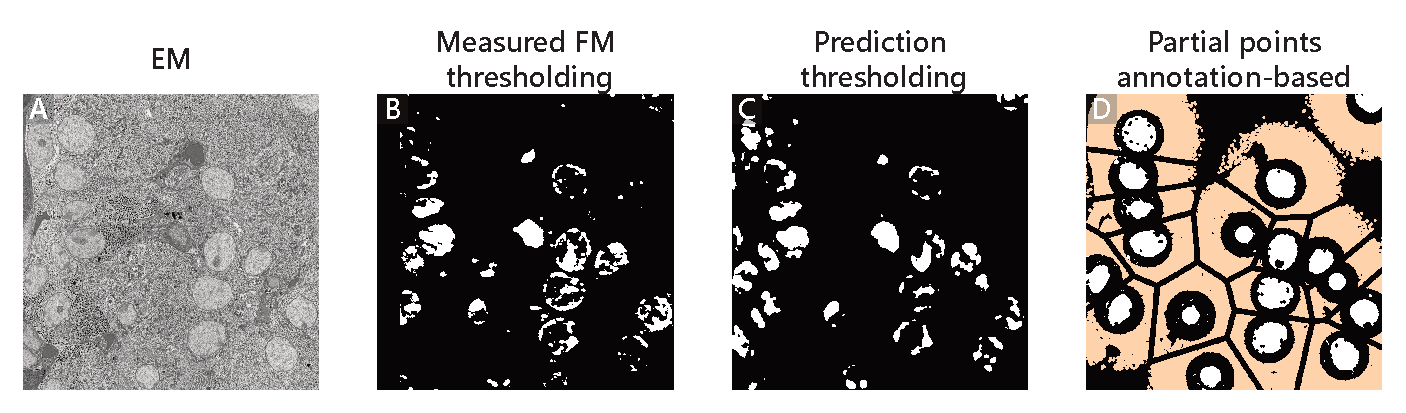
\includegraphics[width=\linewidth]{chapter-4/figures_PDF/fig4-5_masks.pdf}
    \caption{Segmentation masks employed for CNN-based nuclei segmentation.
    (A) (Unlabelled) EM image of cell nuclei.
    (B) Labelled image (segmentation mask) derived from thresholding the correlative image of the measured fluorescence and (C) from thresholding the CLEMnet prediction from (A).
    (D) Segmentation mask derived from a combination of $k$-means clustering and Voronoi partitioning of the corresponding EM image. The points used in the Voronoi partition are the centroids of detected nuclei based on partial points annotation. Labelling scheme in (B\,--\,D): white -- nucleus; black -- background; beige -- unlabelled.}
    \label{fig:4.5_masks}
\end{figure}

We anticipated that the first approach would result in a significant amount of incorrect labels due to the issues mentioned previously (nonspecific labelling, EM-FM registration errors, autofluorescence, etc.). However, because the incorrect labels would be uncorrelated (in the case of EM-FM registration errors) or on featureless areas of the EM (in the case of autofluorescence), we suspected that the model could disregard them to the same extent as was found for the fluorescence predictions (Figure \ref{fig:4.S1_rois}). The more fundamental problem with this simple approach is that the fluorescence signal may not be uniformly distributed throughout an organelle. In cell nuclei, for example, the fluorescence from the Hoechst staining is localized to the nuclear envelope and chromatin-dense subregions. The result from training ResNet-34 on these masks is hence a fragmented segmentation that largely resembles the measured fluorescence itself (Figure \ref{fig:4.6_segmentation}A, ``Measured FM Masks")---nuclei are segmented with high-precision (low FPs), but portions of many nuclei are missed (high FNs). This is in contrast to the segmentation results from the traditional approach of training the network on manually segmented nuclei (Figure \ref{fig:4.6_segmentation}A, ``GT Masks").

% Figure 4.6 (segmentation)
% -------------------------
\begin{figure}[!tb]
    \centering
    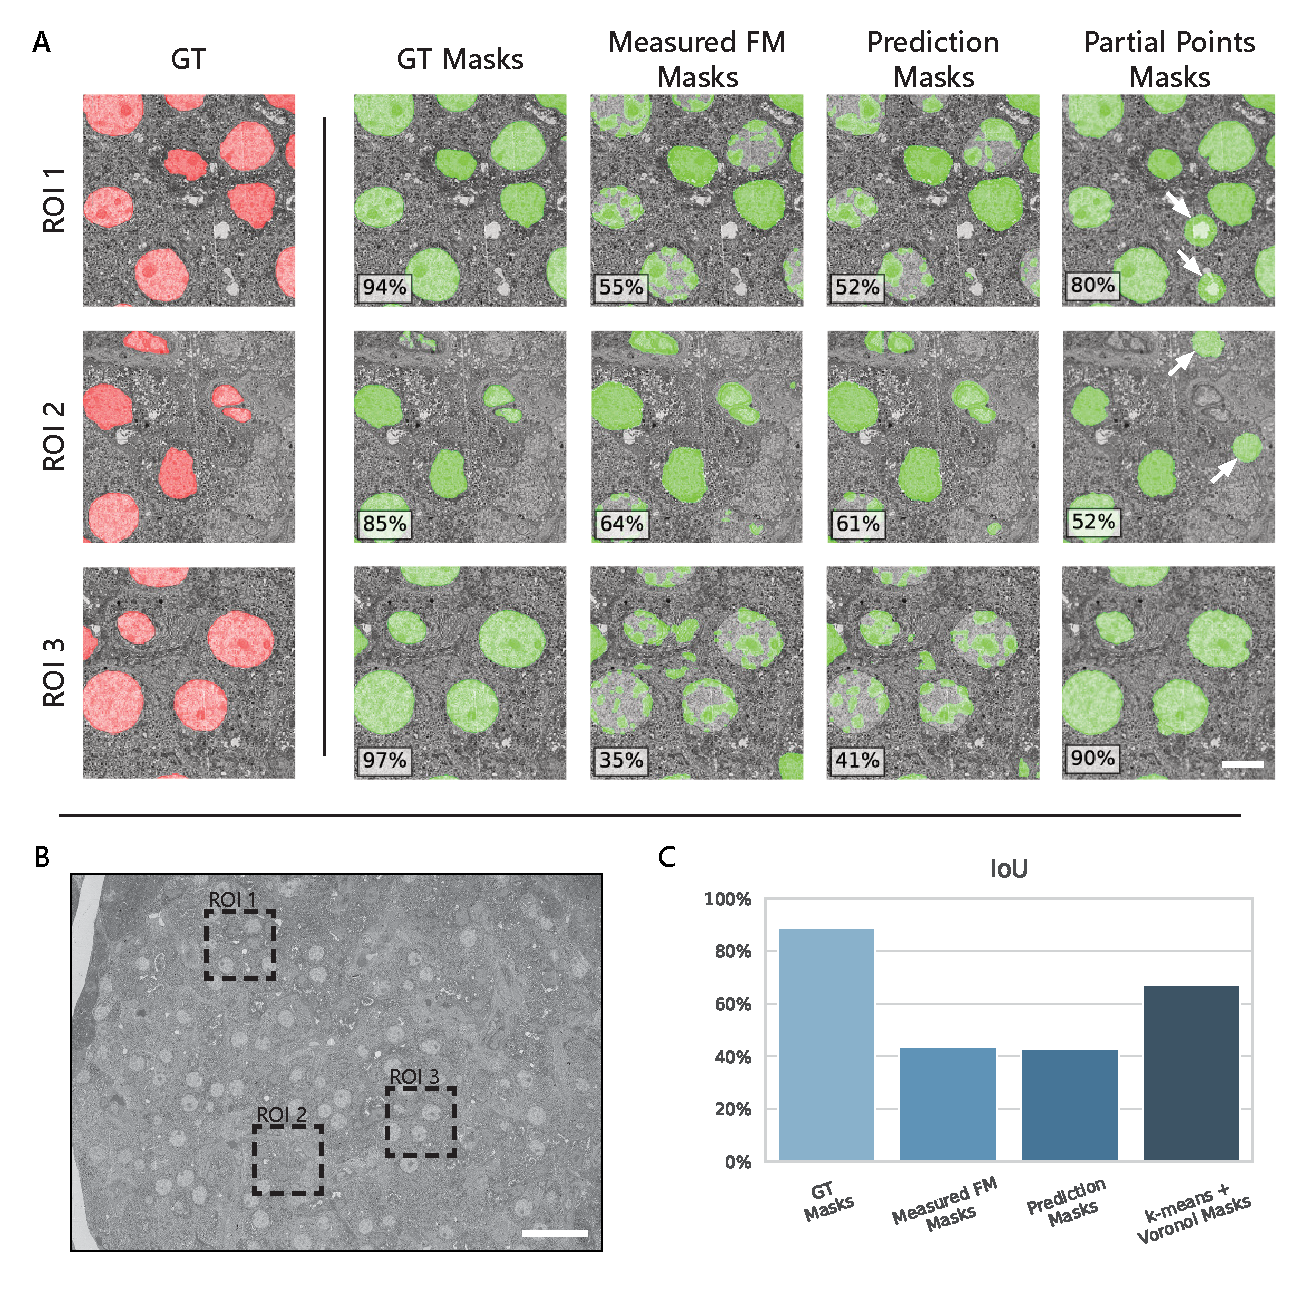
\includegraphics[width=\linewidth]{chapter-4/figures_PDF/fig4-6_segment.pdf}
    \caption{CNN-based segmentation results for various labelling strategies: semi-automated labelling strategy outperforms thresholding approaches.
    (A) Three randomly selected regions of interest are selected from a large-scale EM dataset of rat pancreas tissue (B) to assess segmentation performance. Intersection-over-union (IoU) scores are provided in the corner of each ROI. CNN architecture for all segmentation results is based on ResNet-34. White arrows denote instances of falsely labelled nuclei.
    (C) Aggregate IoU scores of the four segmentation strategies across the entire section. Training on semi-automatically generated segmentation masks derived from partial points annotation together with $k$-means clustering and Voronoi partitioning results in improved segmentation performance.
    Scale bars: (A) \SI{2}{\micro\meter}; (B) \SI{10}{\micro\meter}.}
    \label{fig:4.6_segmentation}
\end{figure}

As CLEMnet was found to predict fluorescence more uniformly throughout the nucleus, we assessed whether generating labelled images by thresholding the CLEMnet predicted data would improve results. The segmentation results (Figure \ref{fig:4.6_segmentation}A, ``Prediction Masks"), however, were comparable to those that derived from thresholding the measured fluorescence data. While some nuclei are flood-filled, reflecting a successful segmentation, these occurrences are highly inconsistent. The intersection over union (IoU) results underscore the vast difference in segmentation performance. IoU scores for ResNet-34 trained on manually segmented nuclei average 89\%, while those for ResNet-34 trained on thresholding the measured fluorescence and CLEMnet predicted signal are 44\% and 43\% respectively (Figure \ref{fig:4.6_segmentation}C).

A more sophisticated approach for generating labelled images was therefore adapted from an approach by \textcite{qu2020weakly} who used partial points annotation to segment cell nuclei from histology images in a weakly supervised fashion. Compared to conventional hand-tracing of organelles, partial point annotation requires only a single point to be selected from a sample of organelles within each image. It thereby constitutes the annotation method requiring the least amount of manual time and effort, while still providing human-assisted supervision. Partial points annotation is particularly advantageous for correlative datasets as the fluorescence overlay facilitates organelle selection by the human annotator. We then trained ResNet-34 on segmentation masks derived from partial points annotations (Figure \ref{fig:4.5_masks}D) as described in Section \ref{sec:4methods_segmentation}. The resulting segmentation performance (Figure \ref{fig:4.6_segmentation}A, ``Partial Points Masks") improved upon the thresholding approaches with an average IoU score of 72\%, despite the presence of some false positives negatives (white arrows). While filtering segments by area would remove the vast majority of these false positives, smaller nuclei---those that were sectioned at the periphery---would also be removed.
